\chapter{Analytic Expressions for the GLE in a Harmonic Well and the Interpretation of GLE parameters} \label{sec:gle_interpretation}

We begin our discussion of the GLE in a background potential in the simple case of a harmonic well of natural frequency $\omega_0$, $V\left(x\right) = \frac{1}{2}m\omega_0^2x^2$. Using the statistical properties of the stochastic force, Appendix \ref{apx:analytic_gle_appendix} provides a first principles derivation of the kinetic energy auto-correlation function and ISF of a particle in a harmonic well with an arbitrary memory kernel. The derivation introduces the Green's function of the GLE denoted $F\left(t\right)$ and the results are quoted in terms of the auto-correlation of the Green's function $C_F(t)$. The general expressions in two dimensions are
\begin{equation}
\left<E(0)E(t)\right>=\frac{\sigma^4}{m^2}\left(\left(\int\frac{dw}{2\pi}\omega^2\left|\tilde{F}(\omega)\right|^2\right)^2 + \left(\int\frac{dw}{2\pi}e^{i\omega t}\omega^2\left|\tilde{F}(\omega)\right|^2\right)^2\right) \label{eq:harmonic_gle_ek}
\end{equation}
\begin{equation}
\left<ISF(\Delta \vec{K}, t)\right> = ISF\left(\Delta \vec{K}, \infty \right)\exp\left(\frac{|\Delta \vec{K}|^2 \sigma^2}{m^2} C_F\left(t\right) \right). \label{eq:harmonic_gle_isf}
\end{equation}
In the particular case of an exponential memory kernel $K(t)=\frac{1}{\tau}e^{-\frac{t}{\tau}}$, these expressions may be evaluated analytically using contour integrals,
\begin{equation}
        ISF\left(\Delta \vec{K}, t\right) = ISF\left(\Delta \vec{K}, \infty\right) \exp\left(\frac{-\sigma^2\left|\Delta \vec{K}\right|^2}{2m^2\tau^2}\left(\frac{e^{-\chi''t}}{2\chi'\chi''}\operatorname{Re}\left(\frac{e^{i\chi't}}{\chi\left(\chi^2+\eta_1^2\right)}\right) + \frac{e^{-\eta_1t}}{\left(\left|\chi\right|^2+\eta_1^2\right)^2\eta_1}\right)\right) \label{eq:exp_isf}
\end{equation}
\begin{equation}
        \left<E(0)E(t)\right>=\left<E(0)E(\infty)\right> + \frac{\sigma^4}{4\tau^4m^2}\left(\frac{e^{-\chi''t}}{2\chi'\chi''}\operatorname{Re}\left(\frac{\chi e^{i\chi't}}{\chi^2+\eta_1^2}\right) + \frac{\eta_1e^{-\eta_1 t}}{\left(\left|\chi\right|^2 + \eta_1^2\right)^2} \right)^2 \label{eq:exp_ek_auto}
\end{equation}
$$
\left<E(0)E(\infty)\right> = \frac{\sigma^4}{4\tau^4m^2}\left(\frac{1}{2\chi'\chi''}\operatorname{Re}\left(\frac{\chi}{\chi^2+\eta_1^2}\right) - \frac{\eta_1}{\left(\left|\chi\right|^2 + \eta_1^2\right)^2} \right)^2.
$$
In the above expressions, $\chi = \chi' + i\chi''$, $-\chi^*$, and $i\eta_1$ are the poles of the Greens function $F(t)$ in the upper half complex plane and are functions of $\omega_0$, $\eta$ and $\tau$. Convolution with an exponential memory kernel is equivelant to a frequency filter of the form $\tilde{H}(\omega) = \frac{1}{1+i\omega t}$ with bandwith $2\pi f_c = \omega_c = \frac{1}{\tau}$. 

While a lot can be said about equations \ref{eq:exp_isf} \& \ref{eq:exp_ek_auto}, for the purposes of this report we simply note that both the kinetic energy auto-correlation function and the ISF exhibit exponentially damped oscillatory behavior parameterized by $\chi'$ and $\chi''$ as well as a pure exponential decay parameterized by $\eta_1$. ISFs generated using GLE parameter values frequently encountered in this report are shown in figure \ref{fig:analytic_isfs}.
 
Figure \ref{fig:pole_parameters} shows contour plots of the parameters $\chi'$, $\chi''$ and $\eta_1$ as a function of $\omega_0$, $\eta$ and $\tau$. In the $\tau \rightarrow 0$ limit these plots demonstrate that $\chi'' \rightarrow \frac{\eta}{2}$, $\chi' \rightarrow \omega_D = \sqrt{\omega_0^2 - \eta^2/4}$ (the frequency of an equivalent under-damped harmonic oscillator) and $\eta_1 \rightarrow \infty$. In this limit, equation \ref{eq:exp_ek_auto} reduces to a form with oscillations of angular frequency $\chi' \approx \omega_D$ and a tail decaying at a rate of $2\chi'' \approx \eta$. This provides a natural interpretation for the oscillations and decay rates in the ISF and energy auto-correlation function of a particle in the small $\tau$ limit. These interpretations will be used as naive estimates for GLE parameters from MD simulation results in later sections and may find a use in extraction of parameters from experimental data. While these results strictly speaking only apply to a harmonic background potential, the potential seen by an adatom at the minimum of an absorption site is well approximated by a harmonic force and so these interpretations remain justified, especially at low temperatures.

\begin{figure}
	\begin{subfigure}{1.0\textwidth}
		\makebox[\textwidth][c]{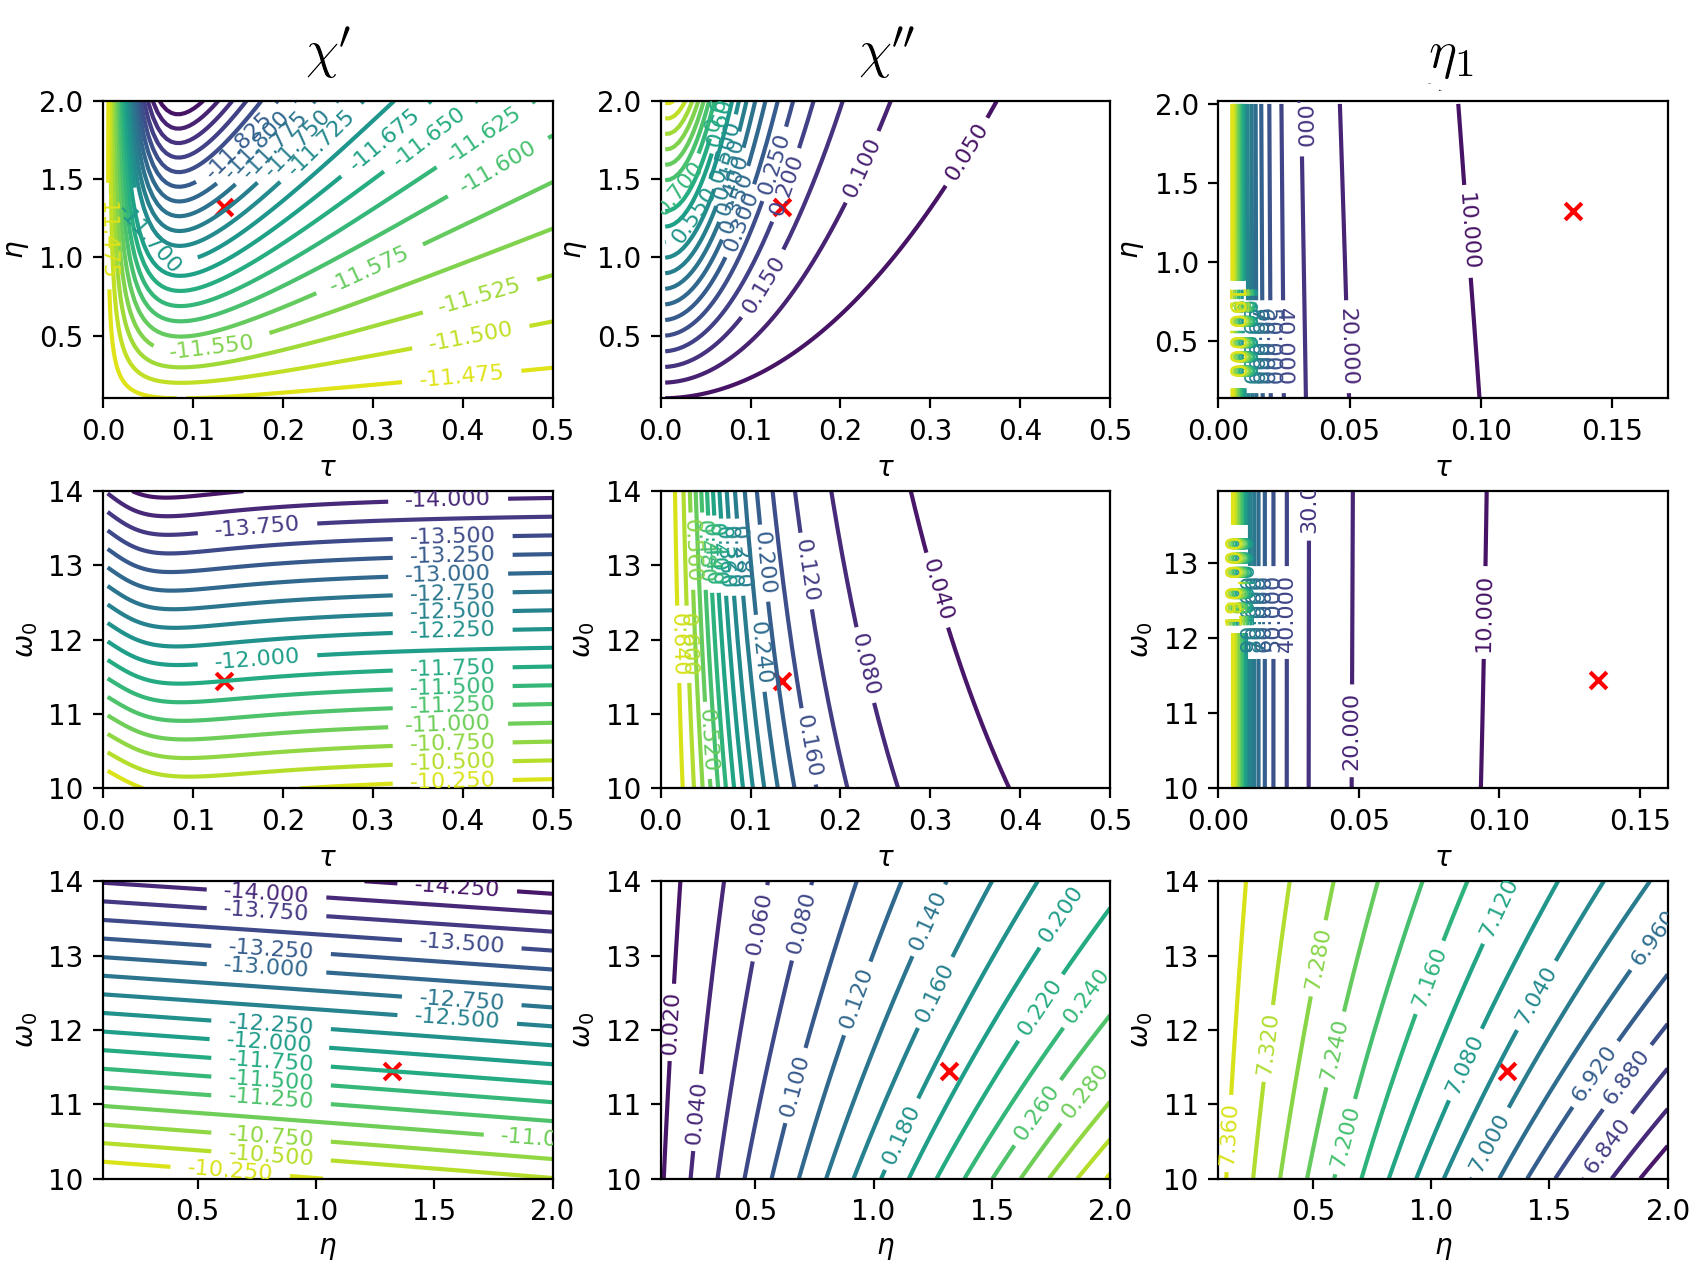
\includegraphics[width=1.2\textwidth]{harmonic_gle_parameters}}
		\caption{Contour plots showing the relationship between the position of the poles of the GLE Green's function and the GLE parameters $\omega_0$, $\eta$ and $\tau$. Each column contains contour plots for one of the pole parameters and the red crosses denote the value of GLE parameters typically encountered in this report.}
		\label{fig:pole_parameters}
	\end{subfigure}

	\begin{subfigure}{1.0\textwidth}
		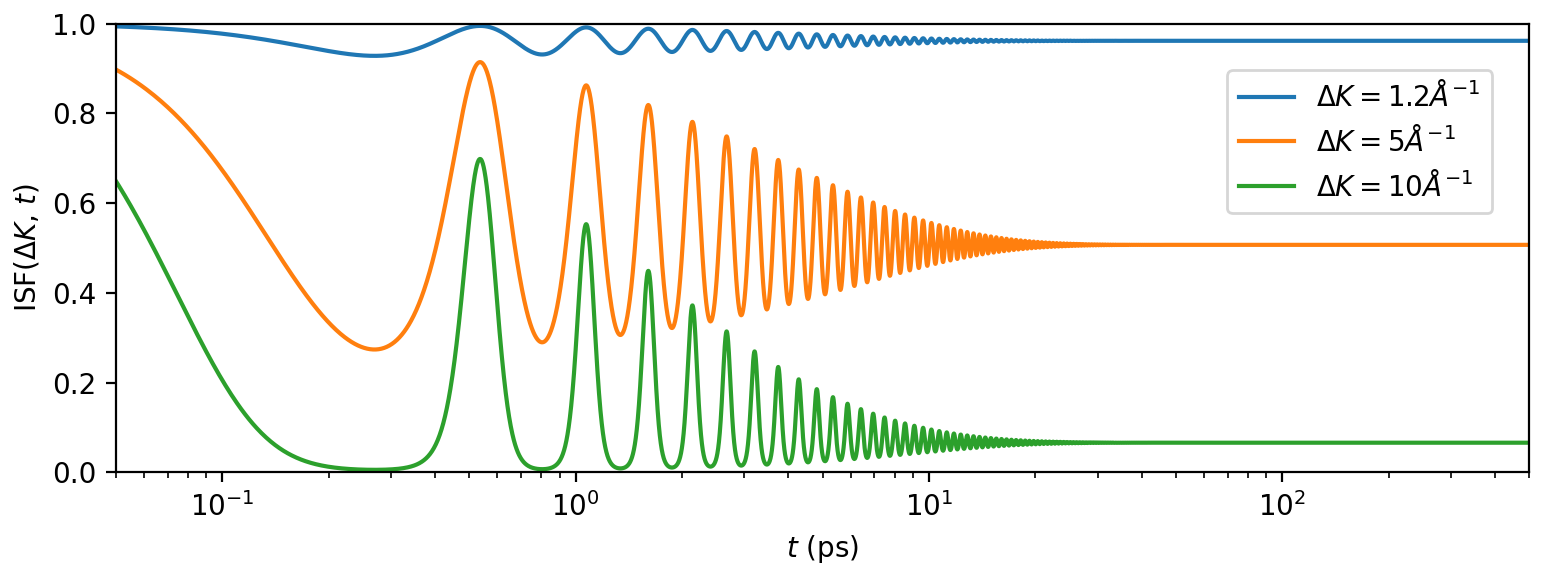
\includegraphics[width=1.0\textwidth]{analytic_isfs}
		\caption{ISFs of a particle in a harmonic potential well of natural frequency $\omega_0=\SI{11.45}{\ips}$ obeying the GLE with parameters $\tau=\SI{0.135}{\ps}$ and $\eta = SI{1.34}{\ips}$ across a range of momentum transfers. Oscillations within the potential well are more pronounced at higher momentum transfers which suggests a means for extracting GLE parameters from experimental data at high momentum transfers.}
		\label{fig:analytic_isfs}
	\end{subfigure}

	\caption{}
\end{figure} 
